\documentclass{article}

\usepackage{lipsum}
\usepackage[margin=1.5in]{geometry}
\usepackage{titlesec}
\usepackage{graphicx}
\usepackage{amsmath}

\usepackage{mathtools, amssymb, nccmath}
\usepackage{bigstrut, changepage, lipsum}

\newcommand{\code}{\texttt}
\newcommand{\norm}[1]{\left\lVert#1\right\rVert}

\usepackage{siunitx} % Required for alignment


% Specify images directory
\graphicspath{ {./report-images/} }

% Header and Footer stuff
\usepackage{fancyhdr}
\pagestyle{fancy}
\fancyhead{}
\fancyfoot{}
\fancyfoot[R]{ \thepage\ }
\renewcommand{\headrulewidth}{0pt}
\renewcommand{\footrulewidth}{0pt}
\newcommand{\sectionbreak}{\clearpage}
\setlength{\parindent}{0pt}

%

\begin{document}

%----------------------------------------------------------------------------------------
%	TITLE PAGE
%----------------------------------------------------------------------------------------

\begin{titlepage} % Suppresses displaying the page number on the title page and the subsequent page counts as page 1
	\newcommand{\HRule}{\rule{\linewidth}{0.5mm}}% Defines a new command for horizontal lines, change thickness here
	
	\center % Centre everything on the page
	
	%------------------------------------------------
	%	Headings
	%------------------------------------------------
	
	\textsc{\Large Random Number Generation and Simulation}\\[0.5cm] % Major heading such as course name
	
	\textsc{\large Exercise 8}\\[0.5cm] % Minor heading such as course title
	
	%------------------------------------------------
	%	Title
	%------------------------------------------------
	
	\HRule\\[0.6cm]
	
	{\huge\bfseries Area estimation using Monte Carlo method}\\[0.25cm] % Title of your document
	
	\HRule\\[1.5cm]
	
	%------------------------------------------------
	%	Author(s)
	%------------------------------------------------
	
	\begin{minipage}{0.4\textwidth}
		\begin{flushleft}
			\large
			\textit{Author}\\
			\textsc{Cesare De Cal} % Your name
		\end{flushleft}
	\end{minipage}
	~
	\begin{minipage}{0.4\textwidth}
		\begin{flushright}
			\large
			\textit{Professor}\\
			\textsc{Annie Cuyt}\\ % Supervisor's name
			[0.25cm]
			\textit{Assistant Professor}\\
			\textsc{Ferre Knaepkens} % Supervisor's name

		\end{flushright}
	\end{minipage}
		
	\vfill\vfill\vfill
	
	{\large\today}
		
	\vfill
	
\end{titlepage}

%----------------------------------------------- Introduction ------------------------------------------------------
\section{Introduction}\label{sec:intro}
The exercise asks to approximate the area of the figure defined by

$$
\begin{cases}
1 \le x \le 3 \\
-1\le y \le 4 \\  
x^3+y^3\le 29 \\
y \ge e^x -2
\end{cases}$$

using the Monte Carlo method.

%---------------------------------- Tools ---------------------------------------------------------------------------
\section{Tools}
To solve this exercise, I've used the following libraries and programming languages:

\begin{itemize}
  \item C
  \item Intel Math Kernel Library (more specifically, the Vector Statistical Library)
  \item OpenMP
  \item C Math Library
\end{itemize}

I've used the following Intel MKL routines:
\begin{itemize}
  \item \code{vslNewStream(\&stream, brng, seed)}
  \item \code{vslLeapfrogStream(stream, k, nstreams)}
  \item \code{vsRngUniform(method, stream, nrRandomNumbers, array, start, end)}
  \item \code{vslDeleteStream(\&streamToDelete)}
\end{itemize}

OpenMP provides a user-friendly interface to build multi-threading applications. I've used the following methods and procedures:
\begin{itemize}
  \item \code{omp\_get\_max\_threads()}
  \item \code{\#pragma omp parallel private(nrOfThreads, threadID)}
  \item \code{omp\_get\_thread\_num()}
\end{itemize}

To make the code more clear, I've also wrote my own function \code{isInsideArea(x,y)} which checks if a given pair of coordinates $(x, y)$ is inside the area drawn by the system of inequalities. To get started with the exercise, I have used the template file \code{template.c} provided on the website.\\

To compile and run the code on my own machine with \code{gcc}, I created a Makefile based on the compiler options and link line specified here:\\ \code{https://software.intel.com/en-us/articles/intel-mkl-link-line-advisor}.

\section{Computation}
On a high level picture, the Monte Carlo method in this exercise works by generating random $(x,y)$ coordinates in the rectangle formed by

$$
\begin{cases}
1 \le x \le 3 \\
-1\le y \le 4 \\  
\end{cases}$$

And then checks if the points satisfy the following inequalities using the \code{isInsideArea(x,y)} function I wrote.

$$
\begin{cases}
x^3+y^3\le 29 \\
y \ge e^x -2
\end{cases}$$

The area is given by the ratio of how many points satisfied the system (in other words, are inside the figure) to the total number of iterations $N$. This is repeated $LOOPS$ times, and finally I calculate the average of all the areas.\\

To make this happen, I created two independent streams of uniformly distributed random numbers.

 

\section{Plots}
%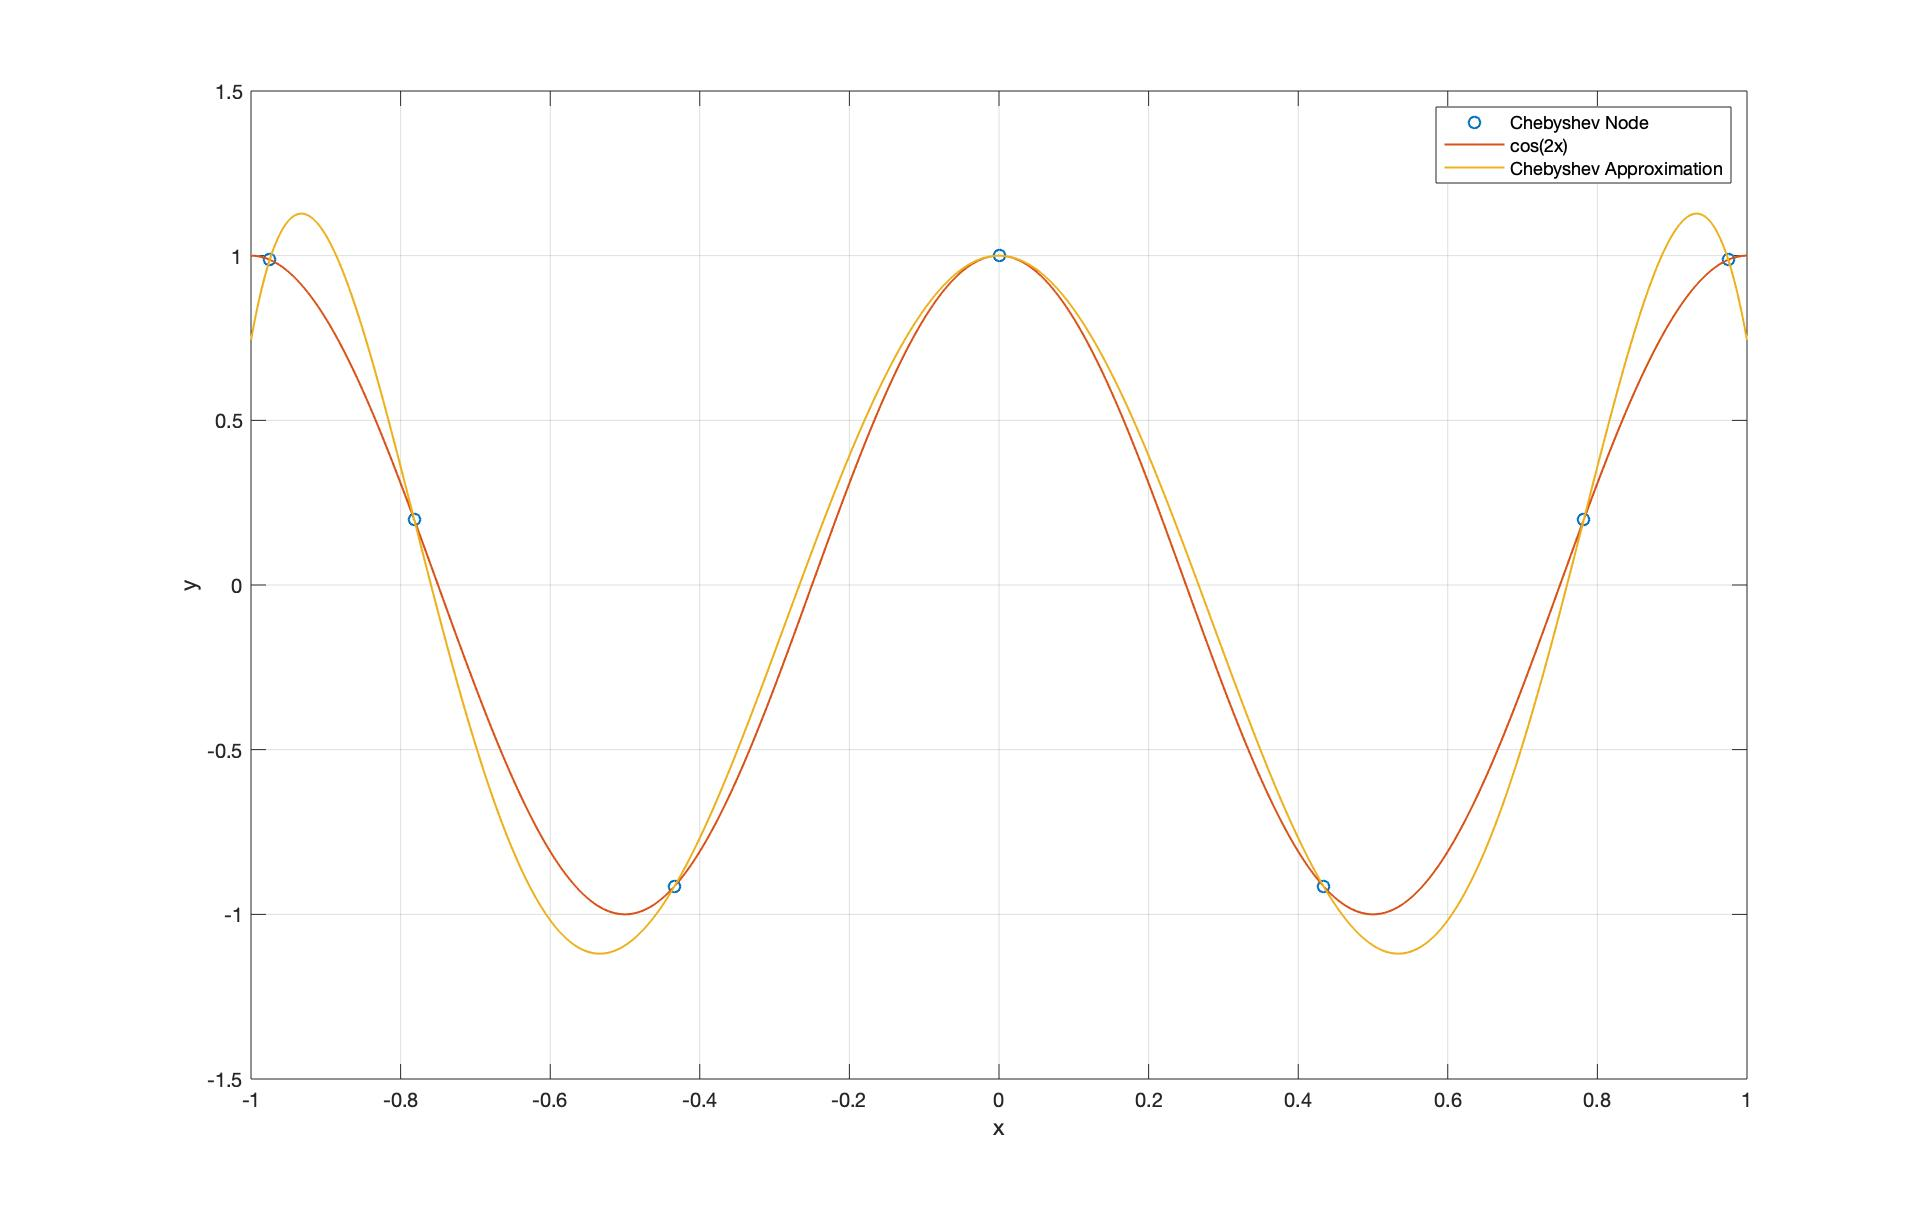
\includegraphics[width=\textwidth,height=\textheight,keepaspectratio]{cos2x.jpg}
%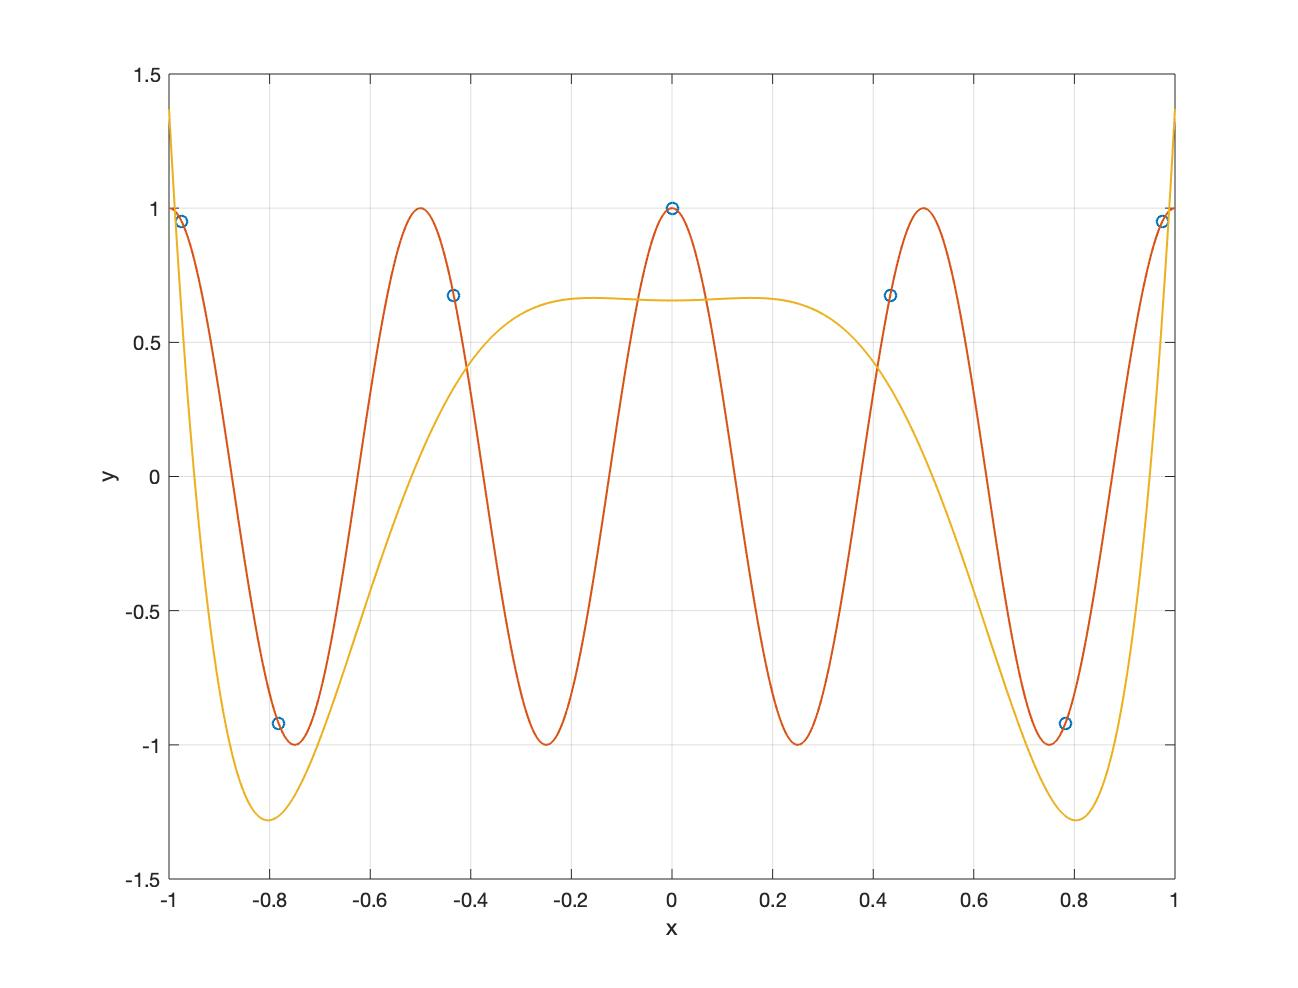
\includegraphics[width=\textwidth,height=\textheight,keepaspectratio]{cos4x.jpg}
\section{Observations}
\end{document}